\section{Methods and Materials}

\subsection{ANTs volumetric-based cortical thickness estimation pipeline}

The ANTs-based cortical thickness estimation workflow is illustrated 
in Figure \ref{fig:pipeline}.  The steps are as follows:
\begin{enumerate}
  \item initial N4 bias correction on input anatomical MRI,
  \item brain extraction using a hybrid segmentation/template-based strategy,
  \item alternation between prior-based segmentation and ``pure tissue'' 
        posterior probability weighted bias correction,
  \item DiReCT-based cortical thickness estimation, and
  \item optional normalization to specified template and multi-atlas
    cortical parcellation. 
\end{enumerate}
Each component, including both software and data, is briefly detailed 
below with the relevant references for additional information. 

%We also note that each component is publicly available with all ANTs 
%algorithms available as open source.%
%\footnote{
%http://www.picsl.upenn.edu/ANTS
%}
The coordination of all the algorithmic components is
encapsulated in the shell script {\tt antsCorticalThickness.sh} with
subcomponents delegated to {\tt antsBrainExtraction.sh} 
and {\tt antsAtroposN4.sh}.  A representative script command 
is reproduced in Listing \ref{listing:antsCorticalThickness} for
a single IXI subject to demonstrate the simplicity and
mature status of what we propose in this work and a comparison
of the analogous FreeSurfer command.  
Option descriptions are provided by invoking the
help option, i.e. `{\tt antsCorticalThickness.sh -h}.'

\lstset{frame = htb,
        framerule = 0.25pt,
        float,
        fontadjust,
        backgroundcolor={\color{listlightgray}},
        basicstyle = {\ttfamily\scriptsize},
        keywordstyle = {\ttfamily\color{listkeyword}\textbf},
        identifierstyle = {\ttfamily},
        commentstyle = {\ttfamily\color{listcomment}\textit},
        stringstyle = {\ttfamily},
        showstringspaces = false,
        showtabs = false,
        numbers = none,
        numbersep = 6pt,
        numberstyle={\ttfamily\color{listnumbers}},
        tabsize = 2,
        language=bash,
        floatplacement=!h,
        caption={\small \baselineskip 12pt ANTs and FreeSurfer command line calls 
        for a single IXI subject which is representative of the calls used for each subject
        of the evaluation study.  
        },
        captionpos=b,
        label=listing:antsCorticalThickness
        }
\begin{lstlisting}
# Processing calls for subject IXI002-Guys-0828-T1

# ANTs
antsCorticalThickness.sh \
  -a IXI/T1/IXI002-Guys-0828-T1.nii.gz \
  -e IXI/template/T_template0.nii.gz \
  -m IXI/template/T_template0ProbabilityMask.nii.gz \
  -p IXI/template/Priors/priors%d.nii.gz \
  -f IXI/template/T_template0ExtractionMask.nii.gz \
  -o IXI/ANTsResults/IXI002-Guys-0828-

# FreeSurfer  
recon-all \
  -i  IXI/T1/IXI002-Guys-0828-T1.nii.gz \
  -s  IXI002-Guys-0828 \
  -sd IXI/FreeSurferResults/ \
  -all
\end{lstlisting}



\begin{figure*}
  \centering
  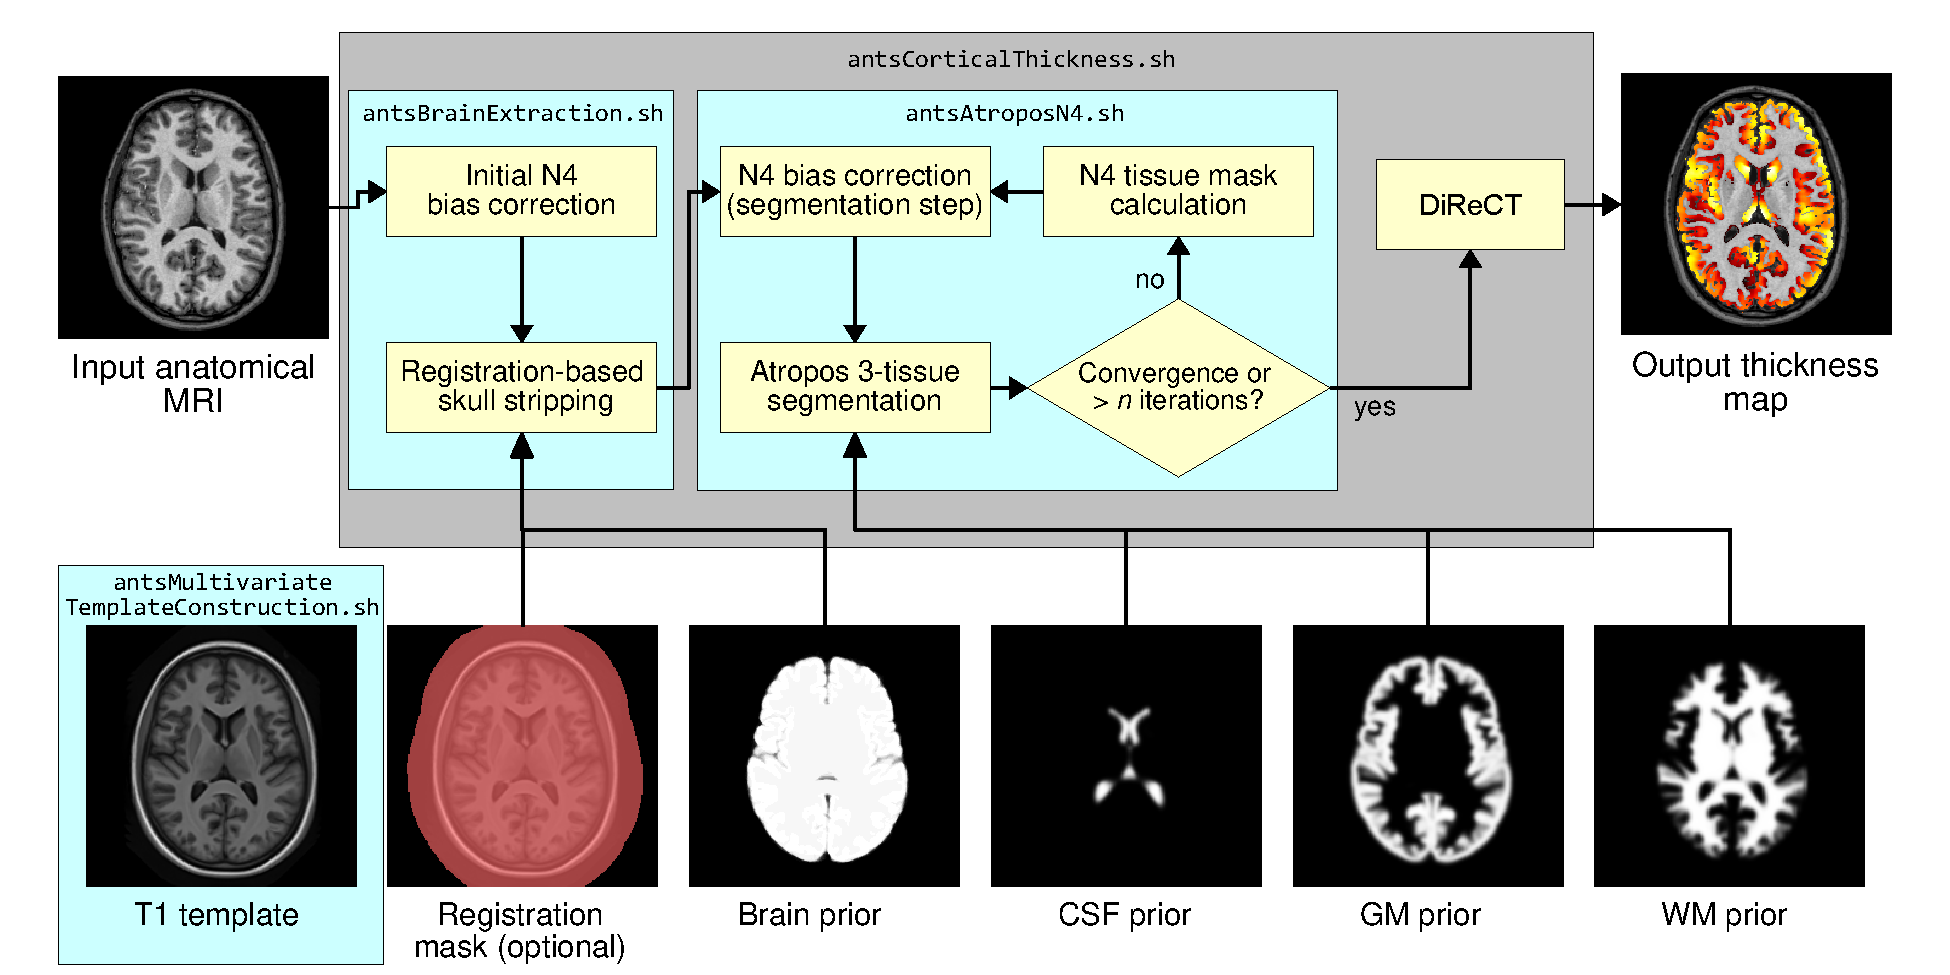
\includegraphics[width=180mm]{Figures/Kapowski_pipeline2.pdf}
  \caption{Illustration of the main components of the ANTs processing 
  workflow containing all elements for determining cortical thickness. 
  We also included the domain of operations for the selected scripts.
  Not shown are the probability maps for the brain stem and cerebellum
  priors.}
  \label{fig:pipeline}
\end{figure*}

\subsubsection{Anatomical template construction}

Normalizing images to a standard coordinate system
reduces intersubject variability in population studies.  Various
approaches exist for determining the normalized space such as the selection
of a pre-existing template based on a single subject, e.g. the Talairach
atlas \citep{Talairach1988}, or a publicly available averaged group of
subjects, e.g. the MNI \citep{Collins1994} or ICBM \citep{Mazziotta1995}
templates.  Additionally, mean templates constructed from labeled
data can be used to construct spatial priors for improving segmentation
algorithms.
The work of \cite{avants2010} explicitly models the geometric component of the 
normalized space during optimization to produce such mean templates.  Coupling the intrinsic symmetry of 
SyN pairwise registration \citep{avants2011} and an
optimized shape-based sharpening/averaging of the template appearance, Symmetric Group
Normalization (SyGN) is a powerful framework for producing optimal population-specific
templates.

The ANTs implementation of this technique is currently available as a shell script, 
{\tt buildtemplateparallel.sh}.  A generalized, multivariate version is also available as
{\tt antsMultivariateTemplateConstruction.sh}.  Both scripts are distributed as part of
 the ANTs repository.
The multivariate script permits the construction of multimodal templates (e.g. 
T1-weighted, T2-weighted, proton density MRI and fractional anisotropy).  
Both scripts accommodate a variety of computational resources
for facilitating template construction.  These computational resource possibilities include:
\begin{itemize}
  \item serial processing on a single workstation, 
  \item parallelized processing on a single workstation with multiple cores using \verb#pexec#%
  \footnote{http://www.gnu.org/software/pexec/pexec.1.html},
  \item parallelized processing using Apple's XGrid technology%
  \footnote{https://developer.apple.com/hardwaredrivers/hpc/xgrid\_intro.html}, 
  \item parallelized processing using Sun Grid Engine for cluster-based systems%
  \footnote{http://www.oracle.com/technetwork/oem/grid-engine-166852.html}, and 
  \item parallelized processing using the Portable Batch System for cluster-based systems%
  \footnote{http://www.pbsworks.com/}.
\end{itemize}

For this work, database-specific templates were used during cortical thickness pipeline
processing for both brain extraction and brain segmentation steps.  Multivariate templates 
were constructed from the multimodal data sets.  However, their usage was based on the 
fact that they had been built previously for other work and not because they provide a 
discernible advantage over univariate templates (i.e. T1-only) for the proposed workflow.

\subsubsection{N4 bias field correction}

Critical to quantitative processing of MRI is the minimization of
field inhomogeneity effects which produce artificial low frequency 
intensity variation across the image.  Large-scale studies, such
as ADNI, employ
perhaps the most widely used bias correction algorithm, N3 \citep{sled1998}, 
as part of their standard protocol \citep{boyes2008}.

In \cite{tustison2010}, we introduced an improvement of N3, denoted as
``N4'', which demonstrates a significant increase in performance and convergence behavior
on a variety of data.  This improvement is a result of an enhanced 
fitting routine (which includes multi-resolution capabilities) and a modified optimization 
formulation.  For our workflow, the additional possibility of specifying
a weighted mask in N4 permits the use of a ``pure tissue'' probability map 
(described below)
calculated during the segmentation pipeline for further improvement of 
bias field estimation.  

N4 is used in two places during the individual subject processing (cf Figure
\ref{fig:pipeline}).  
Initially, it is used to generate an initial bias corrected image for use in
brain extraction.  The input mask is created by adaptively thresholding 
the background from the foreground using Otsu's algorithm \citep{otsu1979}.
Following brain extraction, six-tissue (cerebrospinal fluid, cortical gray 
matter, white matter, deep gray matter, brain stem, and cerebellum)
segmentation involves iterating
between bias field correction using the current pure tissue 
probability map as a weight mask and then using that bias corrected image
as input to the Atropos segmentation step (described below). 

\subsubsection{Brain extraction}

Brain extraction using ANTs combines template building, high-performance
brain image registration, and Atropos with topological refinements.  
An optimal template \cite{avants2010} is first constructed using labeled 
brain data (e.g. LPBA40).  Template construction iterates between estimating
the optimal template and registering each subject to the optimal template.
Thus, the construction produces the transforms necessary to warp each 
subject's labeling to the template space.  We use these transformed labelings
to create a probabilistic estimate of the brain mask for the template.
In this work, we perform the additional step of building separate templates
for each cohort and propagate the probabilistic mask to each cohort template
using registration of the T1-weighted templates (cf Figure \ref{fig:template}).
Further refinement include thresholding the warped brain probability map 
at 0.5 and dilated the resulting mask with a radius of two.  Atropos is used 
to generate an initial three-tissue segmentation estimate within the mask
region.  Each of the three tissue labels undergo specific morphological 
operations which are then combined to create a brain extraction mask for use 
in the rest of the cortical thickness workflow using the script {\tt antsBrainExtraction.sh}.  

A comparison of an earlier version of our extraction methodology 
using open access brain data with publicly available
brain extraction algorithms including AFNI's \verb#3dIntracranial#
\citep{ward1999}, FSL's \verb#BET2# \citep{smith2002}, FreeSurfer's
\verb#mri_watershed# \citep{segonne2004}, and BrainSuite
\citep{dogdas2005} demonstrated that our combined
registration/segmentation approach \citep{avants2010a} performs at the
top level alongside BrainSuite (tuned) and FreeSurfer.

\subsubsection{Atropos six-tissue segmentation}

In \cite{avants2011a} we presented an open source $n$-tissue segmentation software tool
(which we denote as ``Atropos'') attempting to distill 20+ years of active research in this area
particularly some of its most seminal work (e.g. \cite{zhang2001,ashburner2005}). 
Specification of prior probabilities includes spatially varying Markov Random Field modeling, 
prior label maps, and prior probability maps typically derived from our template building 
process.  Additional
capabilities include handling of multivariate data, 
partial volume modeling \citep{shattuck2001}, a memory-minimization mode,
label propagation, a plug-n-play architecture for incorporation of novel likelihood models
which includes both parametric and non-parametric models for both scalar and tensorial
images, and alternative posterior formulations for different segmentation tasks.

Due to the important interplay between segmentation and bias correction,
we perform multiple N4 $\rightleftharpoons$ Atropos iterations.
In order to better integrate Atropos and N4, we use  
a pure tissue probability weight mask generated from the 
posterior probabilities derived from the segmentation 
step.  Given $N$ labels and the corresponding $N$
posterior probability maps $\{ P_1, \ldots, P_N\}$ produced
during segmentation, the N4 weight mask is 
created at each N4 $\rightleftharpoons$ Atropos iteration from
\begin{align}
  P_{pure\,\,tissue}(\mathbf{x}) = \sum_{i=1}^N P_i(\mathbf{x}) \prod_{j=1, j \neq i}^N \left( 1 - P_j(\mathbf{x}) \right).
\end{align}
One of the key insights of the original N3 development is the
observation that inhomogeneities cause the intensity values of
pure tissue peaks to spread in the intensity histogram as though
convolved with a Gaussian.  A core contribution of N3 is the
proposed corrective of deconvolving the intensity histogram to 
accentuate the tissue peaks coupled with a spatial smoothing 
constraint. The pure tissue probability mask
weights more heavily the voxels corresponding to pure tissue 
types (as determined by the segmentation) during the deconvolution process 
while minimizing the contribution of regions such as the gray/white matter 
interface where peak membership is ambiguous. 

Atropos enables prior knowledge to guide the
segmentation process where template-based priors are integrated into the optimization
with a user-controlled weight.  Modulating the likelihood and prior contributions
to the posterior probability is essential for producing adequate segmentations.
Atropos weights the likelihood and priors according to
$P(x|y) \propto P(y|x)^{1-\alpha}P(x)^{\alpha}$
where $\alpha$ is a user-selected parameter which weights the tradeoff between the likelihood and priors terms.
In this work, we chose a weighting of $\alpha = 0.25$ 
based on our extensive experimentation with different parameter weights.

Since cortical thickness estimation only requires the cortical gray
and white matters, the deep gray and white matters 
(both labelings and posterior maps) are combined to a single 
``white matter'' set.  This new set combined with the cortical
gray matter results are the only results from the segmentation
step used in the DiReCT algorithm (described below).  


\subsubsection{DiReCT (aka KellySlater/KellyKapowski) cortical thickness estimation}

DiReCT was introduced 
in \cite{das2009} and made available in ANTs as the program \verb#KellySlater#.
Since then several improvements have been made and incorporated into the program
\verb#KellyKapowski#.%
\footnote{
Traditional academic discourse encountered in the published literature
rarely contextualizes peculiarities such as algorithmic nomenclature.
We briefly mention that
this was the source of a rare disagreement between the first and last authors
based, as many disagreements are, on a simple misunderstanding and not an
affronting existential statement concerning a certain favorite sitcom
of the first author's youth. 
}
Among the most significant advancements is that the more recent
implementation is multi-threaded, written in rigorous ITK coding style, and 
has been made publicly available through  ANTs complete with a unique user 
interface design developed specifically for ANTs tools.  

\subsection{Public data resources}

As mentioned previously, the four public data sets which were processed
using the previously described pipeline are IXI, Kirby, NKI, and Oasis.
In addition, we used a subset of the MindBoggle-101 data%
\footnote{
http://mindboggle.info/data.html
} 
labeled using the 
Desikan-Killiany-Tourville (DKT) protocol \citep{klein2012} to define the
regions of interest (ROI).
All five data sets are described below.

\subsubsection{MindBoggle-101 data for ROI definitions}

In \cite{klein2012}, the authors proposed the DKT protocol---a modification of the 
popular Desikan protocol \cite{desikan2006} for purposes of labeling
consistency and facilitating FreeSurfer cortical classification of 
regions. This work resulted in a publicly available set of 101 DKT-labeled T1-weighted 
brain images from different sources including a subset of 20 images
from the Oasis data set which we use to define volumetric regions for each subject
during the ANTs processing.  Since the regional thickness values defined by the DKT atlas 
are calculated as part of the current FreeSurfer processing protocol, this atlas 
provides the common measurement standard for comparison between ANTs and FreeSurfer.

Cortical label propagation to each individual subject for all data sets
described below was performed using the PICSL multi-atlas joint label fusion
algorithm described in \cite{wang2013} with parameters used in the script
{\tt antsMalfLabeling.sh}
which is also distributed with the ANTs toolkit.  
Cortical thickness values are averaged
within each label for each subject using only the non-zero voxels 
from the cortical thickness map. 

\begin{table}
\centering
\begin{tabular*}{0.475\textwidth}{@{\extracolsep{\fill}} l l}
\toprule
  1) caudal anterior cingulate & 2) caudal middle frontal \\
  3) cuneus & 4) entorhinal \\
  5) fusiform & 6) inferior parietal \\
  7) inferior temporal & 8) isthmus cingulate \\
  9) lateral occipital & 10) lateral orbitofrontal \\
  11) lingual & 12) medial orbitofrontal \\
  13) middle temporal & 14) parahippocampal \\
  15) paracentral & 16) pars opercularis \\
  17) pars orbitalis & 18) pars triangularis \\
  19) pericalcarine & 20) postcentral \\
  21) posterior cingulate & 22) precentral \\
  23) precuneus & 24) rosterior anterior cingulate \\
  25) rostral middle frontal & 26) superior frontal \\
  27) superior parietal & 28) superior temporal \\
  29) supramarginal & 30) transverse temporal \\
  31) insula & {} \\  
\bottomrule
\end{tabular*}
\caption{The 31 cortical labels (per hemisphere) of the DKT atlas.  }
\label{table:dkt_labels}
\end{table}


\subsubsection{Public data for thickness estimation evaluation}

\begin{figure}
  \centering
  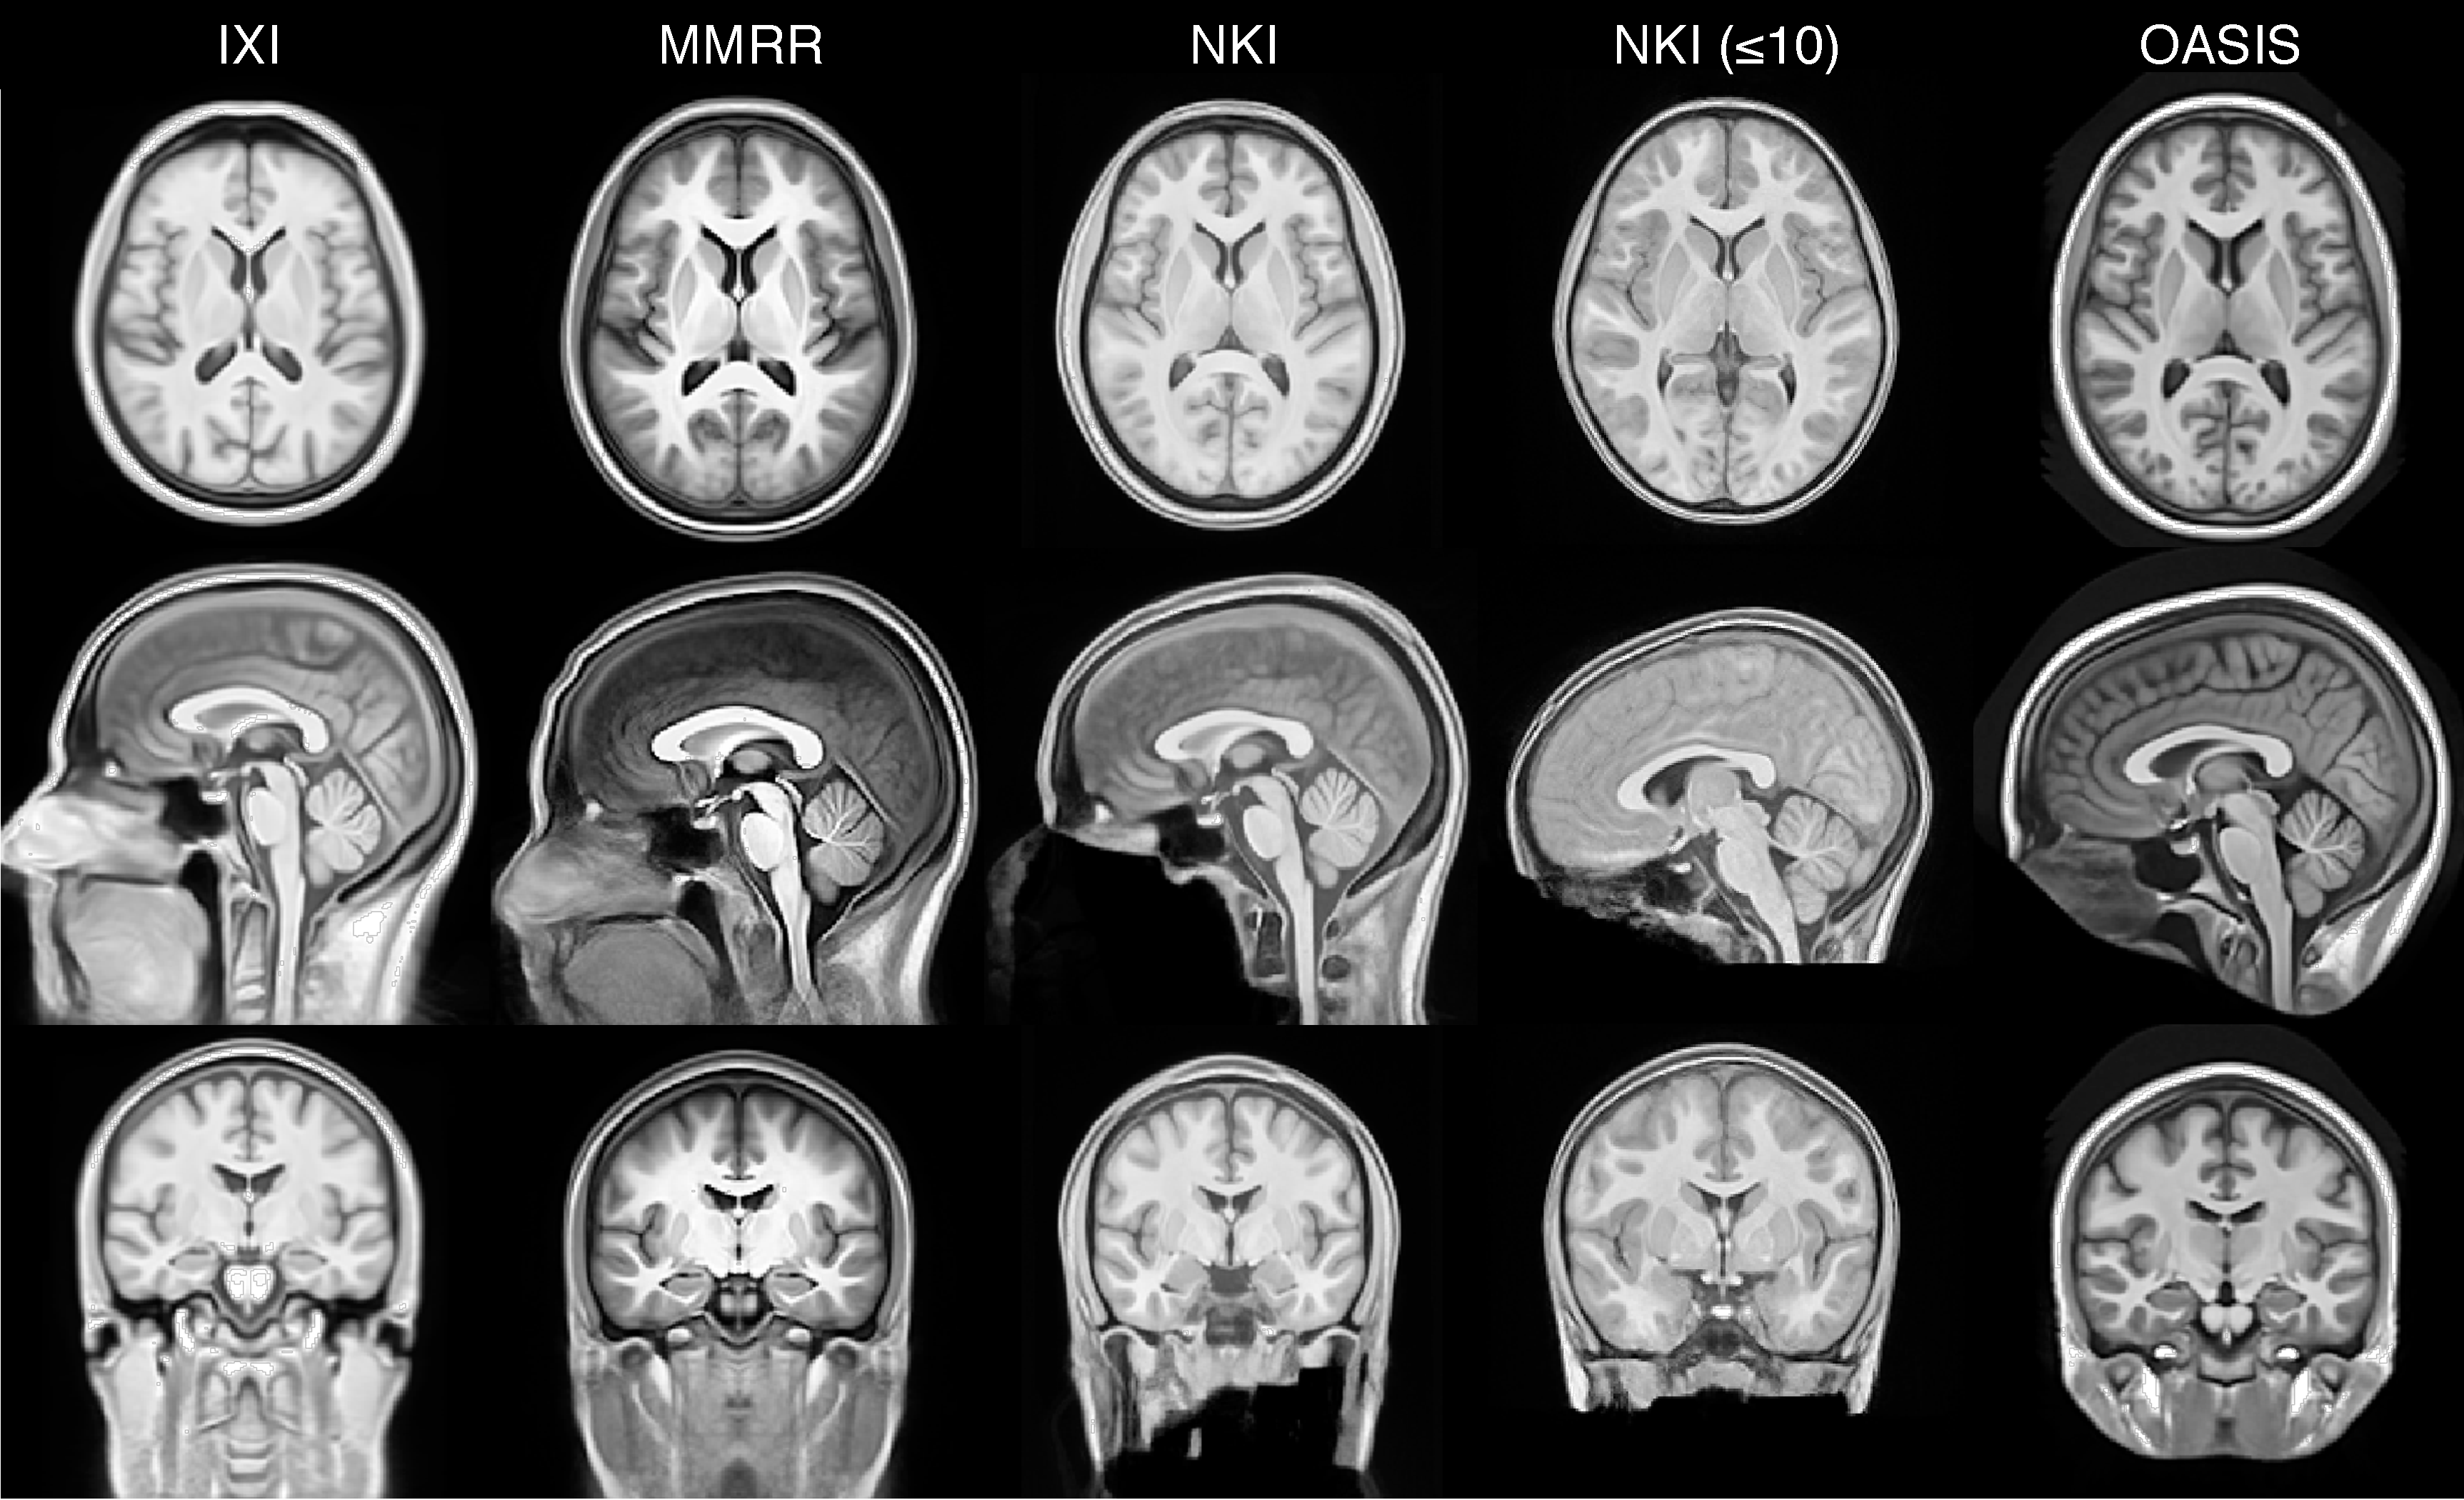
\includegraphics[width=90mm]{Figures/templates.pdf}
  \caption{Population-specific templates for each of the four public data sets used 
  for cortical thickness 
  estimation generated using the script {\tt antsMultivariateTemplateConstruction.sh}. 
  The benefit of using such templates is obvious considering the variability in
  acquisition and data preparation (e.g. defacing protocols).
  }
  \label{fig:template}
\end{figure}

We apply the same pipeline to diverse publicly available datasets collected
from multiple sites and with a mixture of 3T and
1.5T T1 brain images.  Subjects in this dataset
span the age range from 4 to 96 years old.  This strategy tests robustness to
variation in head position, brain shape, defacing, image contrast, inhomogeneity, imaging
artifacts, and the broad variation in extracerebral tissue.  Failure
can occur in initial brain extraction, segmentation, registration, or
bias correction, any of which will lead to an inaccurate cortical
thickness measurement.                           

In total, we processed 1205 T1-weighted images from four different
public data sets to obtain the corresponding cortical thickness maps.                           
The descriptions of the four data sets are as follows: 
                                          
\paragraph{IXI}
Initially, we began with 581 T1-weighted images from the IXI%
\footnote{
http://biomedic.doc.ic.ac.uk/brain-development/
}
 data set
of which all were processed but only 563 subjects 
(313 females, 250 males) were included in the post processing analysis due to 
missing demographic information preventing an accurate estimate of 
the age at the time of image acquisition.  These data were
imaged at three sites 
with several modalities acquired (T1-weighted, T2-weighted, proton density, magnetic 
resonance angiography, and diffusion tensor imaging).  The 
database also consists of  demographic information such as date of birth, date
of scan, weight,
height, ethnicity, occupation category, educational level, and marital status.

\paragraph{Kirby}
The Multi-Modal MRI Reproducibility Resource%
\footnote{
http://www.nitrc.org/projects/multimodal/
}, 
or more informally, the Kirby
data set, was originally described in \cite{landman2011} consisting of 
21 subjects (10 females, 11 males) and features a rich multiple modality and 
repeated acquisition schedule.

\paragraph{NKI}
In support of open science, the 1,000 Functional Connectomes Project%
\footnote{ 
http://fcon\_1000.projects.nitrc.org
}
was initiated on December 11, 2009 by various members of the MRI community
seeking to form collaborative partnerships with imaging institutions for 
sharing well-documented multimodal image sets accompanied by phenotypic data.
One such contribution is the Nathan Klein Institute (NKI)/Rockland sample
consisting of 186 T1-weighted
images (87 females, 99 males).%
\footnote{
Downloaded on September 22, 2012.
}

\paragraph{Oasis}
The initial Open Access Series of Imaging Studies (OASIS)%
\footnote{
http://www.oasis-brains.org/
}
data set consisted of 433 T1-weighted images.  All were processed
although 100 subjects were excluded from analysis due to probable Alzheimer's
disease ($CDR > 0$) and 20 subjects had repeat scans
for 313 individual subjects included in the normal group statistical
analysis (118 males, 195 females).
Ages were between 18 and 96 and  
all subjects are right-handed.  
%Additional processing is included
%with the distribution including bias corrected and segmented images
%(gray, white and CSF matters).  


\begin{figure}
  \centering
  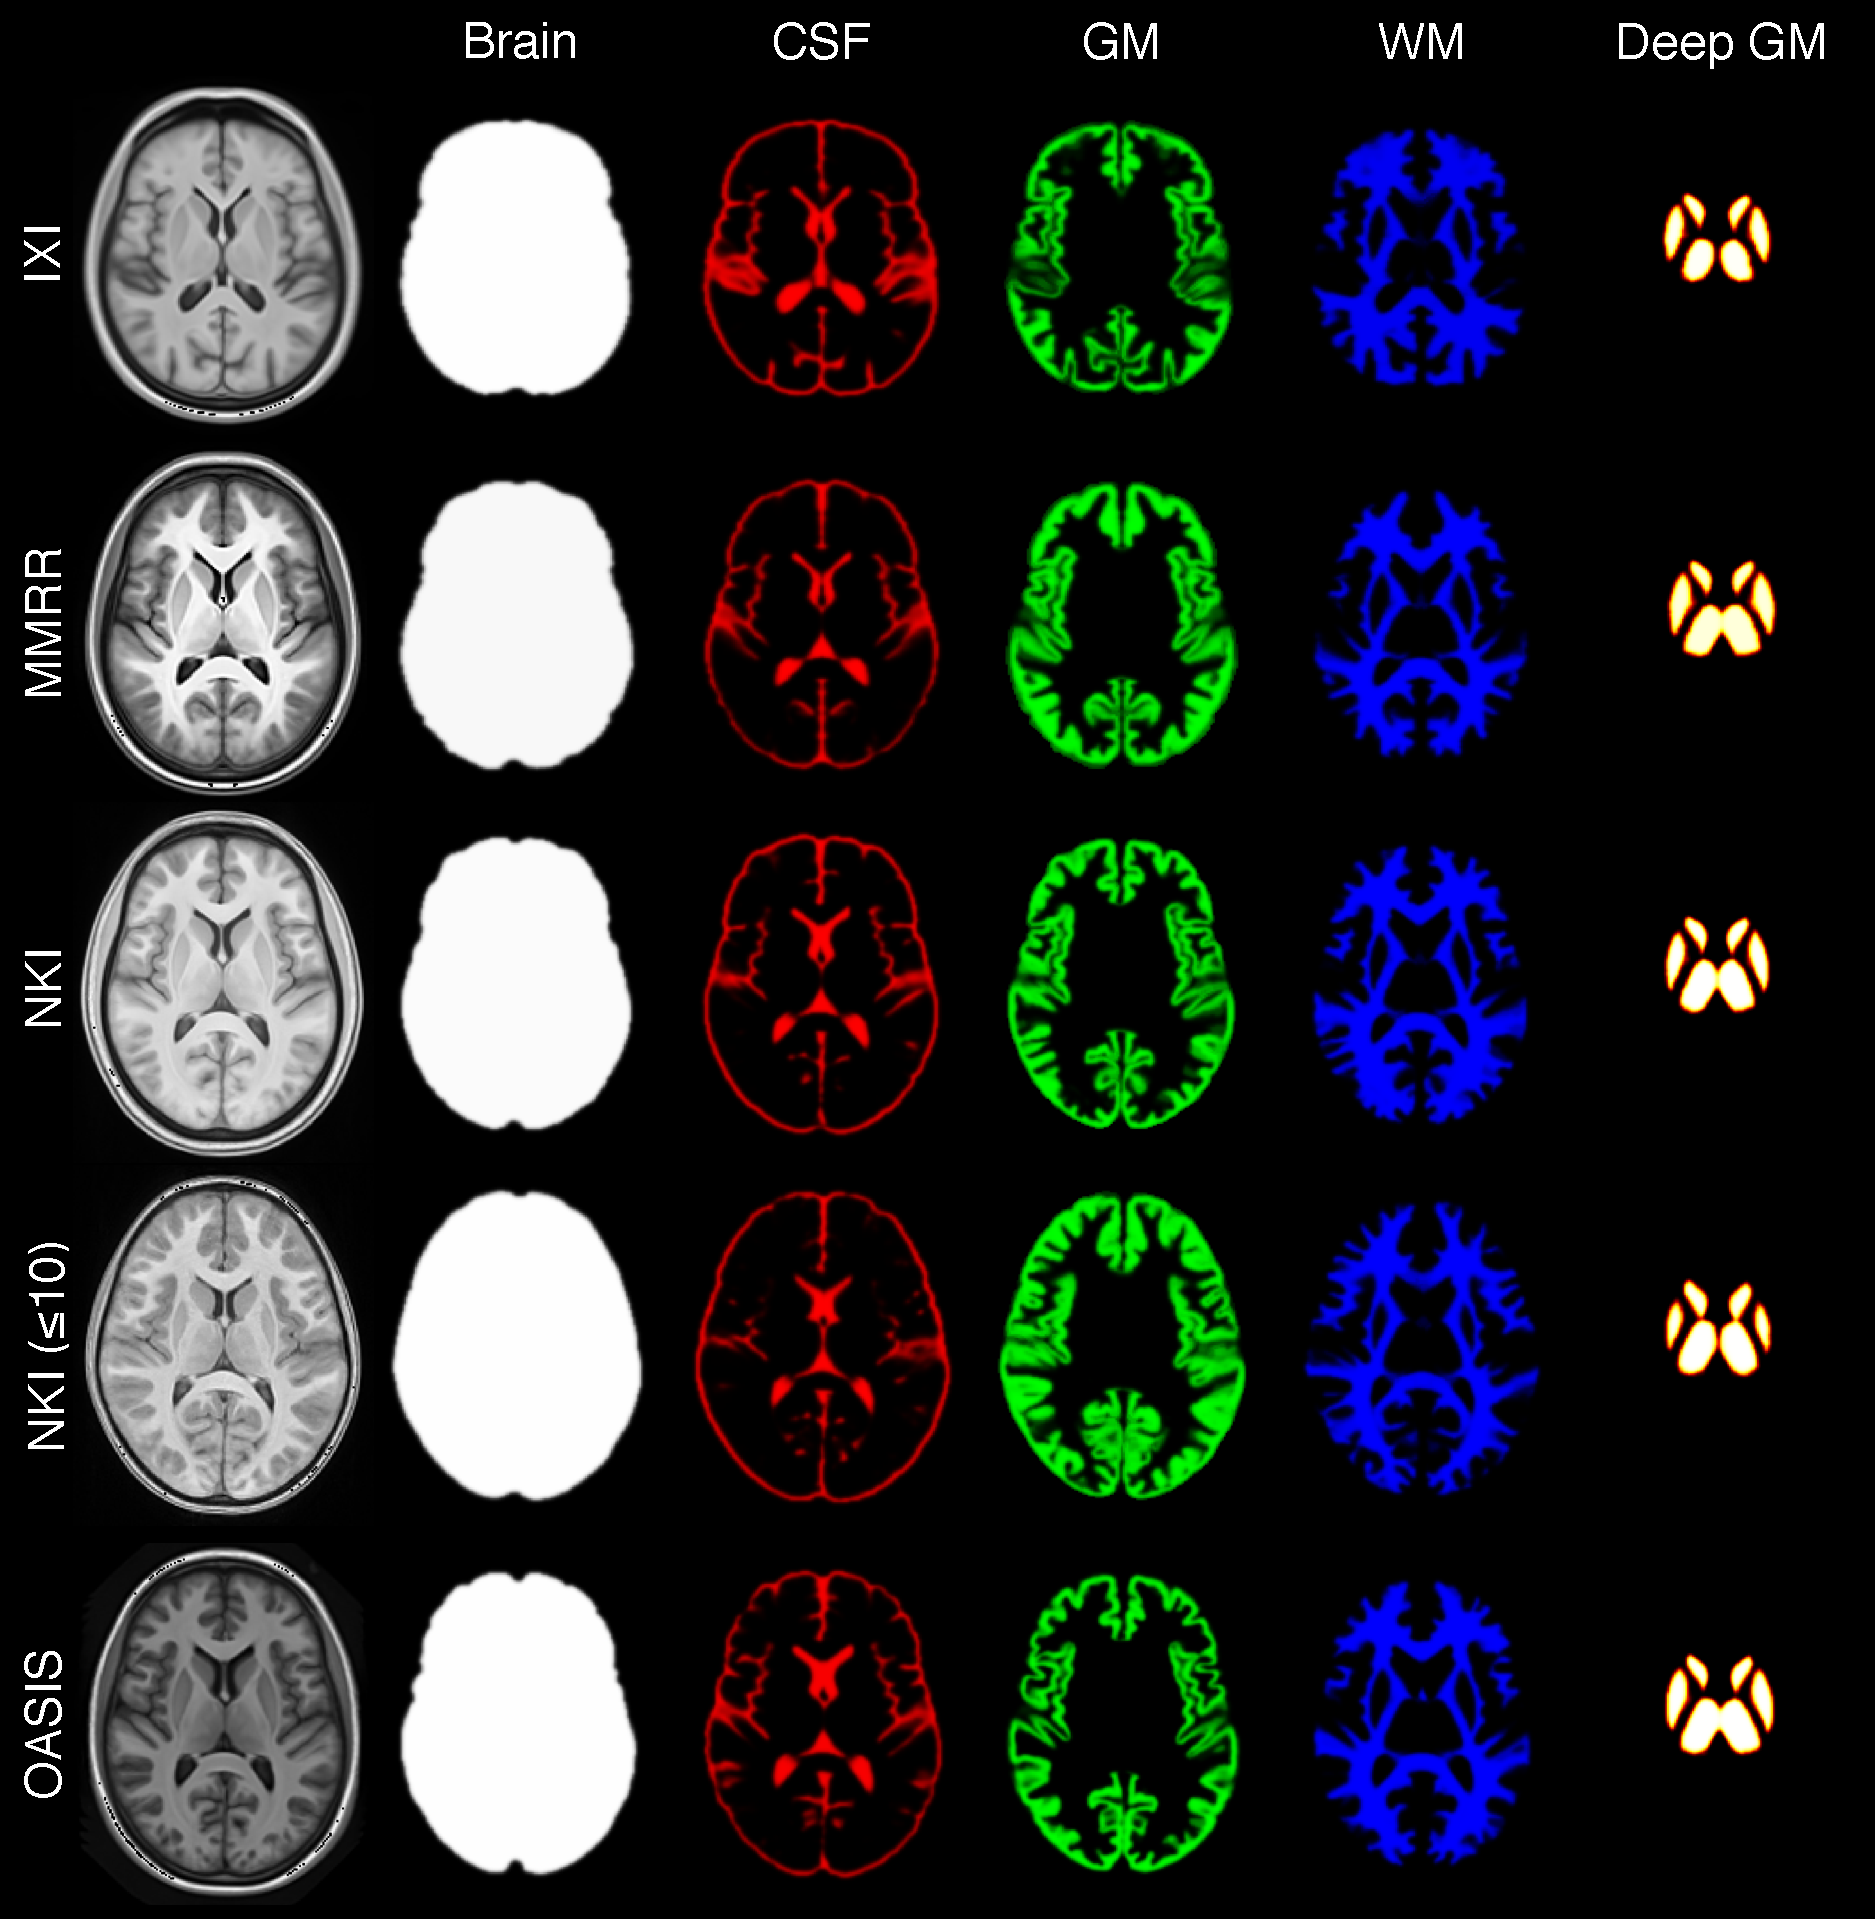
\includegraphics[width=90mm]{Figures/templateProbabilityMasks.pdf}
  \caption{Axial slices from each of the five T1 templates including the corresponding
  probability masks used for brain extraction and brain tissue segmentation.  Not shown
  are the prior probability maps for brain stem and cerebellum regions.
  }
  \label{fig:templateMasks}
\end{figure}


\subsection{Processing miscellany}

Given the documented variability in FreeSurfer results with version number and
Mac OS \cite{gronenschild2012} (as we would expect with our own ANTs pipeline), 
all data was processed using the same ANTs and FreeSurfer versions on the same 
hardware platform.  Processing was performed using the Linux (CentOS release 6.4) 
cluster at the University 
of Virginia%
\footnote{
http://www.uvacse.virginia.edu/
}
using single-threading with a maximal requested memory footprint of 8 Gb for ANTs 
and 4 Gb for FreeSurfer.  The development version of ANTs was used for processing 
(git commit tag: 69d3a5a6c7125ccf07a9e9cf6ef29f0b91e9514f, date Dec. 11, 2013).  
FreeSurfer version 5.3 x86\_64 for CentOs was downloaded 
on 5 December, 2013 (``freesurfer-Linux-centos6\_x86\_64-stable-pub-v5.3.0'', release
date: 15 May, 2013). 


